\documentclass[]{standalone}
\usepackage{siunitx}
\usepackage{tikz}
\begin{document}
  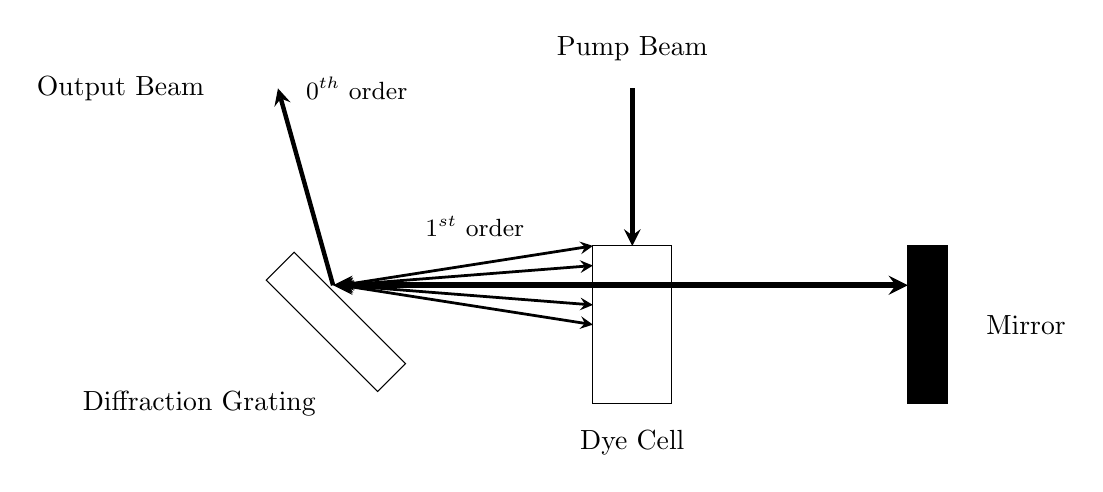
\begin{tikzpicture}
	%Cell
	\draw (0,0) rectangle (1,2);
	\node(dyecell) at (.5,-.5) {Dye Cell};
	%mirror
	\draw[fill = black] (4,0) rectangle (4.5,2);
	\node(mirror) at (5.5,1) {Mirror};
	% Grating
	\draw[rotate around = {45:(-3.3,1)}] (-3.5,0) rectangle (-3,2);
	\node(grating) at (-5,0) {Diffraction Grating};
	%input beam
	\draw[->,>=stealth, line width = 1.6pt] (.5,4) -- (.5,2);
	\node(input) at (.5,4.5) {Pump Beam};
	%Lasing beam
	\draw[<->,>=stealth, line width = 2.0pt] (-3.3,1.5) -- (4,1.5);
	\draw[<->,>=stealth, line width = 1.0pt] (-3.2,1.5) -- (0,2.0);
	\draw[<->,>=stealth, line width = 1.0pt] (-3.2,1.5) -- (0,1.75);
	\draw[<->,>=stealth, line width = 1.0pt] (-3.2,1.5) -- (0,1.25);
	\draw[<->,>=stealth, line width = 1.0pt] (-3.2,1.5) -- (0,1.00);
	%output beam
	\draw[->,>=stealth, line width = 1.6pt] (-3.3,1.5) -- (-4,4);
	\node(output) at (-6,4) {Output Beam};
	\node(oth) at (-3,4) {\small$0^{th}$ order};
	\node(1st) at (-1.5,2.25) {\small$1^{st}$ order};


  \end{tikzpicture}
\end{document}
